\subsection{Programmstruktur}
\label{subsec:programmstruktur}


Im folgenden Abschnitt wird die genaue Struktur des Programmcodes dargestellt, um mit dieser die in den folgenden
Unterkapiteln zu beschreiben und der Gesamtstruktur besser zuordnen zu können.
Die Programmstruktur folgt dem in Unterkapitel \ref{fig: Grundlegende Strukturmuster des Applikations-Ordners} beschriebenen Strukturmuster.
Eine genaue Beschreibung der Struktur des Programmcodes.
Struktur und der Inhalt der Ordner werden in der folgenden Abbildung \ref{fig: Genaue Struktur des Applikations-Ordners} dargestellt.
Die in der Abbildung vorkommenden Daten entsprechen genau den der Anwendung.


\begin{figure}[H]
    \centering
    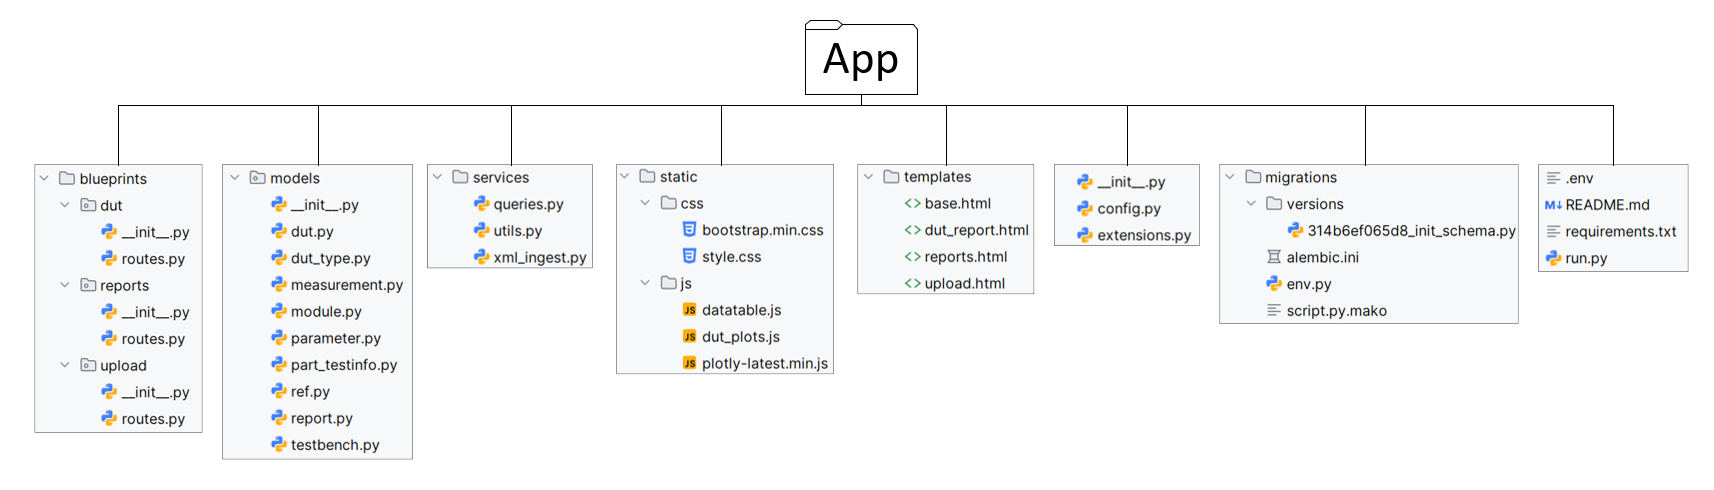
\includegraphics[width=1\textwidth]{Grafiken/Min Ordnerstruktur Projekt.png}
    \caption{Genaue Struktur des Applikations-Ordners}
    \label{fig: Genaue Struktur des Applikations-Ordners}
    {Quelle: Eigene Darstellung mit Microsoft Visio}
\end{figure}